\section{问题分析}

\subsection{总体思路}

四个问题共享同一套物理对象与同一组物理约束，差别只在两处：\textbf{决策时刻能获得哪些信息}，以及\textbf{计划与实际不一致时如何结算}。因此本文采用“\emph{一个物理内核 $+$ 四条信息集主线}”的建模框架：先把母线能量平衡、储能状态转移、容量与功率限值、弃光上界写成与问题无关的公共约束组，再对每一问仅替换目标函数中的费用项、扩展决策变量的维度（是否引入调整量），并重新界定信息集。这样做的直接好处是：四问的模型结构完全一致，结论之间的差异可以精确归因，不会出现口径漂移（这正是 2021 年 C 题评阅要点中唯一被红字强调的失分点——各期方案必须随前一期的状态动态变化，而不能用一套静态方案贯穿始终）。

具体地，问题 1 是完全信息下的确定性经济调度，用于验证物理约束与求解器；问题 2 在\textbf{完全无法获得当天预报}的极端信息集下，仅用历史观测构造因果预测，并把 $5$ 倍紧急电价转化为非对称损失；问题 3 引入官方多时刻预报，形成“$0{:}00$ 基准计划 $\rightarrow$ 每 $6$ h 滚动调整 $\rightarrow$ 实际执行 $\rightarrow$ 状态递推”的闭环；问题 4 只把电价序列换成逐日逐时的波动电价，用于检验前两类策略在价格波动下的稳健性。

整体技术路线如图~\ref{fig:overall-technical-route} 所示。

% 整体技术路线图（由 paper-diagram Skill 绘制的 .drawio 导出 PNG）
\begin{figure}[htbp]
	\centering
	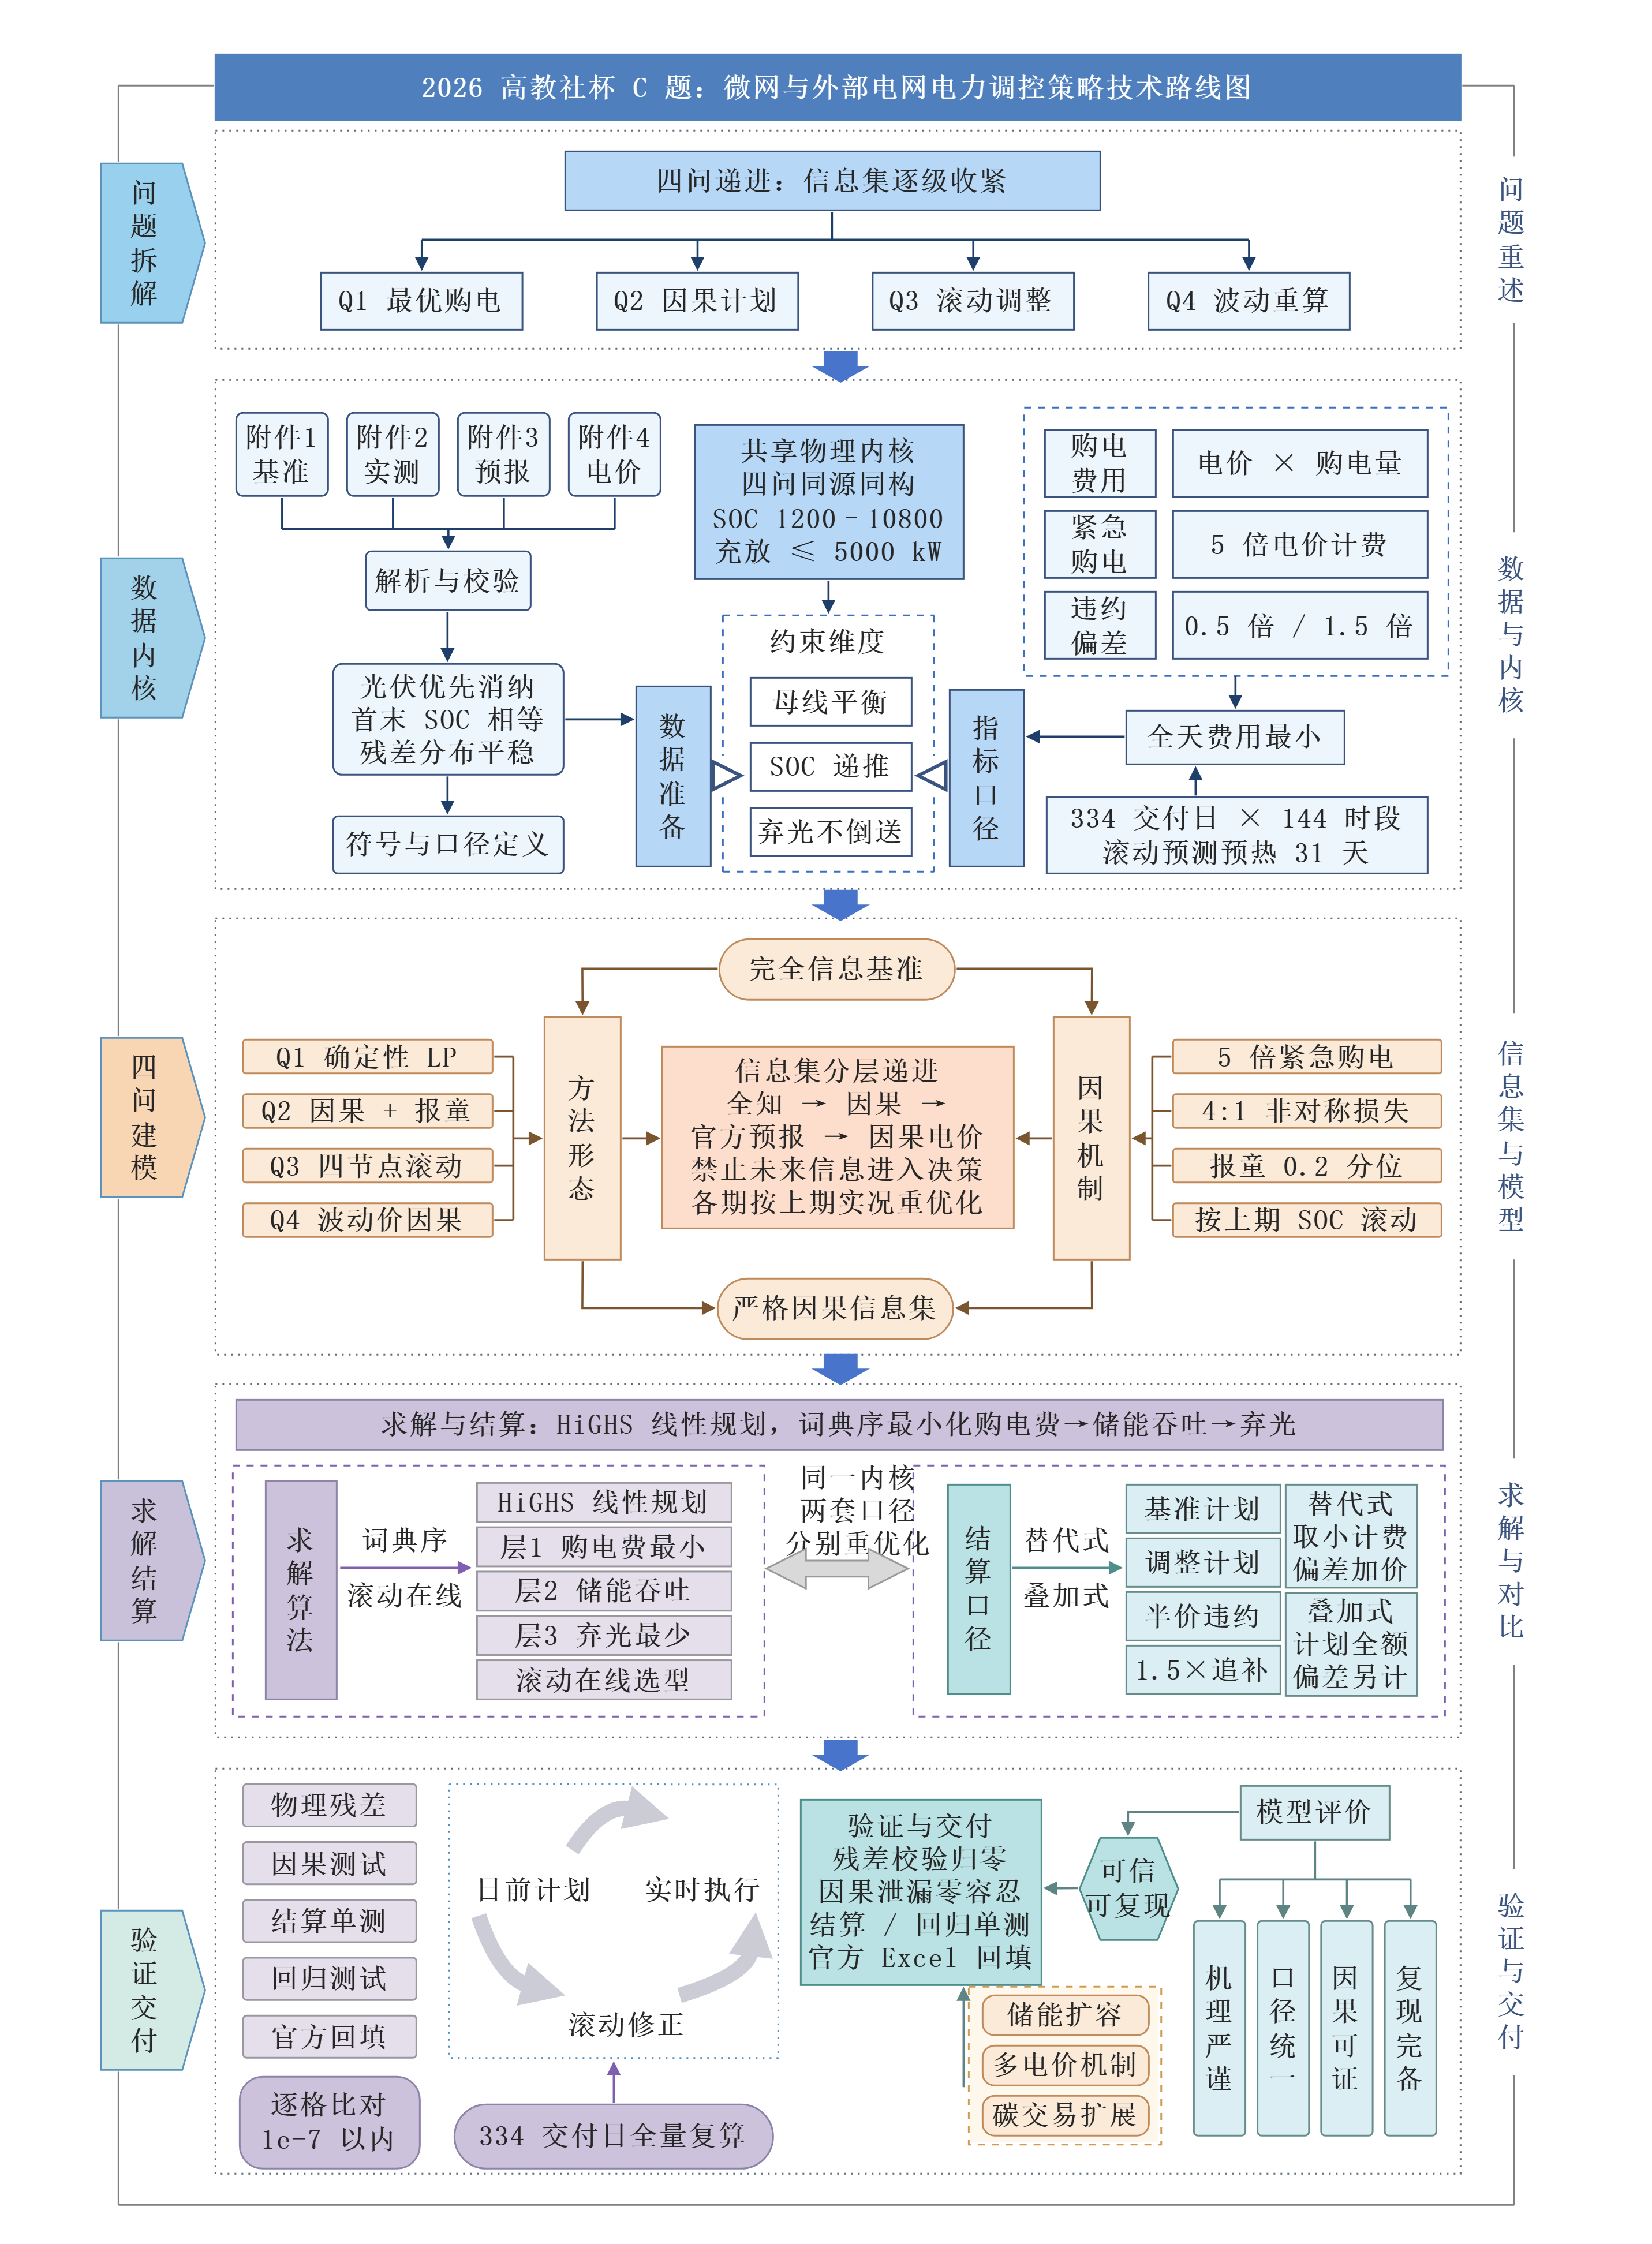
\includegraphics[width=0.98\textwidth]{figures/technical_route.png}
	\caption{整体技术路线图}
	\label{fig:overall-technical-route}
\end{figure}


\subsection{各问的具体分析}

\noindent \textbf{问题一的分析}。题目给定电价、负载与光伏发电功率预测，且“每天的电价和小区负载相同”，因此属于确定性优化。需要注意两个物理细节：其一，附件 2 中存在光伏功率高于负载的时段，若不允许弃光，模型将不可行，因此必须设置弃光变量；其二，题目要求 $0{:}00$ 与 $24{:}00$ 储电量相同，该闭环条件会改变最优解的取值，必须作为硬约束显式写入。

\noindent \textbf{问题二的分析}。本问的信息集最弱：题目没有给出任何当天预报，只能依赖已经发生的历史观测。这与问题一有本质区别——若仍沿用当天真实数据，紧急购电将几乎不会触发，模型退化为问题一。因此必须构造只使用历史数据的因果预测器，并让预测误差真实地转化为远高于计划成本的紧急购电费用。$5$ 倍电价是本问的切入点：它使“高估光伏”的边际损失是“低估光伏”的 $4$ 倍，二者的不对称性决定了最优预测应当偏向保守一侧。此外，由于计划在 $0{:}00$ 锁定且日内不再修改，实际偏差只能依靠储能进行 $10$ min 级的实时缓冲。

\noindent \textbf{问题三的分析}。本问引入了 $6{:}00$、$12{:}00$、$18{:}00$ 三个新增预报时刻，题目据此询问“是否需要引入”。回答这一问有两种做法：一是比较不同降尺度／校正方法的费用，二是把“允许使用的预报节点集合”本身作为消融变量。前者只能回答“哪种处理方法更好”，后者才能回答“这些预报值多少钱”。本文采用后者，构造 $S_0$（仅 $0{:}00$）$\to S_1$（$+6{:}00$）$\to S_2$（$+12{:}00$）$\to S_3$（$+18{:}00$）四组对照，每组保持负载预测方式、降尺度方法、结算口径、终端策略与实时反馈完全一致，只改变可用预报节点，从而得到每一时刻的\textbf{增量价值}。同时，题目的费用结构存在两种合理解释（计划与调整取差额结算，或计划费与调整费叠加），二者会导出不同的目标函数，因而\textbf{最优调度本身也不同}，必须分别完整重新优化而不能只做事后换算式计费。

\noindent \textbf{问题四的分析}。本问只替换电价序列。附件 4 的电价在日内与日间均大幅波动（全天最低 $0.0076$ 元/kWh，最高 $1.7936$ 元/kWh），峰谷价差显著扩大，为储能套利创造了更大空间。但价格序列本身同样构成信息边界：若在 $0{:}00$ 优化时直接读入当天 $144$ 个真实电价，就重演了问题二中的“未来信息穿越”。因此本文把价格也纳入信息集分层，分别给出“价格完全已知”（理想化下界）与“因果价格预测”（可实现）两类结果，其差额即为电价信息的价值。

\subsection{求解框架}

全部四问均归结为线性规划，统一采用 HiGHS 单纯形／内点混合求解器求解。为避免线性规划在大规模最优面上返回无经济意义的退化解（例如同一时段既充电又放电），本文设计三层词典序目标：第一层优化真实费用，第二层在费用容差带内最小化储能吞吐量，第三层再最小化弃光量。统计口径上，所有电量均按 $10$ min 时段能量（kWh）核算，功率与能量的换算系数为 $\Delta t=1/6$ h。
